\section[Frameworks]{Digital Libraries frameworks}\index{Digital Libraries!Frameworks}
\label{sec:background:reference-models-frameworks}

A reference model is an abstract framework that provides basic concepts used to understand the relationships among items in an environment. The \gls{oasis} \citep{MacKenzie2006}⁠ states that a reference model consists of a minimal set of unifying concepts, axioms and relationships within a particular problem domain, and is independent of specific standards, technologies, implementations or other concrete details.

Several \gls{dl} frameworks \citep{Gonccalves2004,Kahn2006} and reference models \citep{Candela2007a} have addressed specific problems in \gls{dls} architectural design and implementation. A discussion of some prominent reference models now follows.

%\subsection{Warwick Framework}
%\label{sec:background:reference-models-frameworks:warwick}
%
%Xxx xxx
%
%Xxx xxx
% @comment: Clearly, this right here is not in anyway relevant.
%
\subsection[5S framework]{Streams, Structures, Spaces and Societies}
\label{sec:background:reference-models-frameworks:5s}

The \gls{5s} framework\index{Digital Libraries!Frameworks!5S} is a unified formal theory for \glspl{dl}. It is an attempt to define and easily understand the complex nature of \glspl{dl} in a rigorous manner. The framework is based on formal definitions, and abstraction of five fundamental concepts---Streams, Structures, Spaces, Scenarios and Societies \citep{Gonccalves2004}⁠.  The five concepts, together with their corresponding definitions and examples, are summarised in Table~\ref{tab:background:reference-models-frameworks:5s}.

\tablespacing
%%%%%\begin{longtable}{p{0.15\linewidth} p{0.40\linewidth} p{0.30\linewidth}}
\begin{longtable}{
>{\arraybackslash}p{0.15\linewidth}|
>{\arraybackslash}p{0.40\linewidth}|
>{\arraybackslash}p{0.30\linewidth}}

\caption{Summary of key aspects of the 5S framework}
\label{tab:background:reference-models-frameworks:5s} \\
 %%%%%\toprule
 %%%%%\hline
 \textbf{Concept} & \textbf{Description} & \textbf{Examples} \\
 %%%%%\midrule
 \cline{1-3}
 \endfirsthead
 
 \caption[]{(continued)}\\
 %%%%%\toprule
 %%%%%\hline
 \textbf{Concept} & \textbf{Description} & \textbf{Examples} \\
 %%%%%\midrule
 \cline{1-3}
 \endhead
 
 % Page footer
 %%%%%\midrule
 %%%%%\hline
 \multicolumn{3}{r}{(Continued on next page)} \\
 \endfoot
 
 % Last page footer
 %%%%%\bottomrule
 \endlastfoot
 
 \textbf{Streams} &
 {Streams represent a sequence of elements of an arbitrary type} &
 {Text, video, audio, software} \\
 
 \cline{1-3}
 %\cmidrule[0.1pt](l{0.5em}r{0.5em}){1-3}
 
 \textbf{Structures} &
 {Structures specify the organisation of different parts of a whole} &
 {Collection, document, metadata} \\
 
 \cline{1-3}
 %\cmidrule[0.1pt](l{0.5em}r{0.5em}){1-3}
 
 \textbf{Spaces} &
 {Spaces are sets of objects, with associated operations, that obey certain constants} &
 {User interface, index} \\
 
 \cline{1-3}
 %\cmidrule[0.1pt](l{0.5em}r{0.5em}){1-3}
 
 \textbf{Scenarios} &
 {Scenarios define details for the behaviour of services} &
 {Service, event, action} \\
 
 \cline{1-3}
 %\cmidrule[0.1pt](l{0.5em}r{0.5em}){1-3}
 
 \textbf{Societies} &
 {Societies represent sets of entities and the relationships among them} &
 {Community, actors, relationships, attributes, operations} \\
 
\end{longtable}

\bodyspacing

In the context of the aims of \glspl{dl}, Gon\c{c}alves et al. \citep{Gonccalves2004} outline an association between \gls{5s} and some aims of a \gls{dls}, with Streams being aligned with the overall communication and consumption of information by end users; Structures supporting the organisation of information; Spaces dealing with the presentation and access to information in usable and effective ways; Scenarios providing the necessary support for defining and designing services; and Societies defining how a \gls{dl} satisfies the overall information needs of end users.

However, Candela et al. \citep{Candela2007}⁠ state that the \gls{5s} framework is very general-purpose and thus less immediate. The \gls{5s} framework is also arguably aimed at formalising the \gls{dl} aspects, as opposed to prescribing specific design guidelines.

\subsection[Kahn\& Wilensky framework]{Kahn and Wilensky framework}
\label{sec:background:reference-models-frameworks:kahn-wilensky}

This is a generic information system framework for distributed digital object services with digital objects as the main building blocks. The framework is based on an open architecture that supports large and distributed digital information services. Kahn and Wilensky\index{Digital Libraries!Frameworks!Kahn/Wilensky} \citep{Kahn2006}⁠ describe the framework in terms of the fundamental aspects of an open and distributed infrastructure, and how the basic components in such an infrastructure support storage, accessibility and management of digital objects.

In addition to a high level conceptual description of such a distributed information system, the framework primarily focuses on the network-based aspects of such an infrastructure \citep{Kahn2006}. Specifically, an elaborate description of how digital objects should be accessed via a \gls{rap} is outlined. The framework also proposes the use of a handle server infrastructure as a means for mapping registered digital objects.

In essence, the framework merely prescribes conventional methods for the unique identification, reliable location, and flexible access to digital objects.

\subsection{DELOS reference model}
\label{sec:background:reference-models-frameworks:delos}

The DELOS\index{Digital Libraries!Frameworks!DELOS} Network of Excellence on \glspl{dl}\footnote{\url{http://www.delos.info}} was a European Union co-funded project aimed at integrating and coordinating research activities in \glspl{dl}. The DELOS working group published a manifesto that establishes principles that facilitate the capture of the full spectrum of concepts that play a role in \glspl{dl} \citep{Candela2007a}⁠. The result of this project was a reference model---the DELOS \gls{dl} reference model---comprising to a set of concepts and relationships that collectively attempt to capture various entities of the \gls{dl} universe.

A fundamental part of the DELOS reference model is the \gls{dl} Manifesto, that presents a \gls{dl} as a three-tier framework consisting of a \gls{dl}, representing an organisation; a \gls{dls}, for implementing \gls{dl} services; and a \gls{dlms}, comprising of tools for administering the \gls{dls}. Figure~\ref{fig:background:reference-models-frameworks:delos}\footnote{Permission to reproduce this image was granted by Donatella Castelli} shows the interaction among the three sub-systems.

The reference model further identifies six core concepts that provide a firm foundation for \glspl{dl}. These six concepts---Content, User, Functionality, Quality, Policy and Architecture---are enshrined within the \gls{dl} and the \gls{dls}. All concepts, with the exceptions of the Architecture concept, appear in the definition of the \gls{dl}. The Architecture is, however, handled by the \gls{dls} definition \citep{Candela2007}⁠.

The Architecture component, addressed by the \gls{dls}, is particularly important in the context of this research as it represents the mapping of the functionality and content on to the hardware and software components. Candela et al. \citep{Candela2007}⁠ attribute the inherent complexity of \glspl{dl} and the interoperability challenges across \glspl{dl} as the two primary reasons for having Architecture as a core component.

Another important aspect of the reference model, directly related to this research, are the reference frameworks needed to clarify the \gls{dl} universe at different levels of abstraction. The three reference development frameworks are: Reference Model, Reference Architecture, and Concrete Architecture. In the context of architectural design, the Reference Architecture is vital as it provides a starting point for the development of an architectural design pattern, thus paving the way for an abstract solution.

\begin{figure}
 %\begin{center}
  \centering
  \framebox[\textwidth]{%
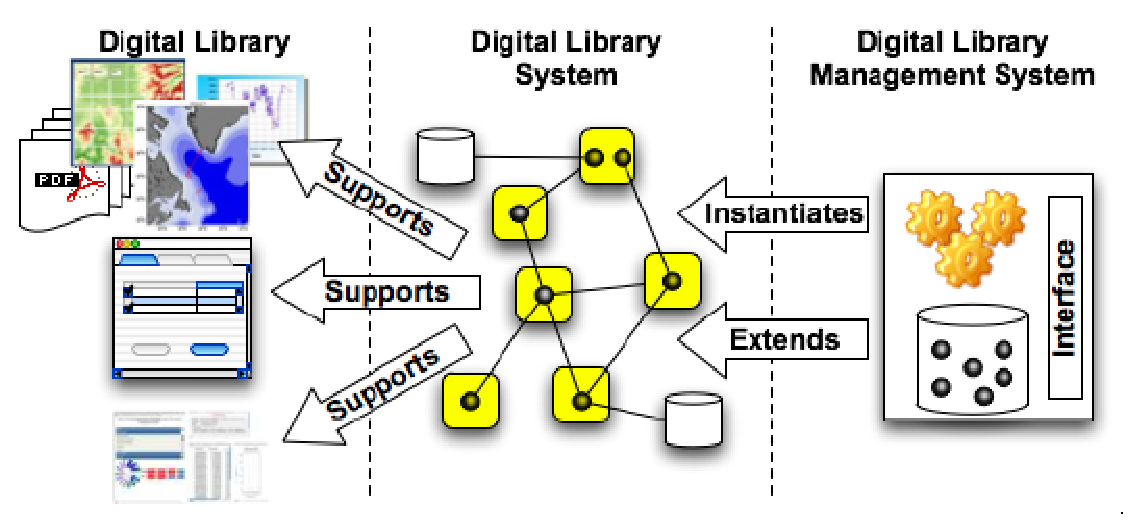
\includegraphics[width=0.95\textwidth]{%
chapter02/figures/delos-dl-dls-dlms.eps}%
}%
\caption[DL, DLS and DLMS: A three-tier framework]{DL, DLS and DLMS: A three-tier framework}
\label{fig:background:reference-models-frameworks:delos}
% \end{center}
\end{figure}

\subsection{Summary}
\label{sec:background:reference-models-frameworks:summary}

The motivation behind building both the reference models was largely influenced by the need to understand the complexity inherent in \glspl{dl}. The idea of designing a \gls{dl} architecture based on direct user needs is not taken into account in existing reference models, although the DELOS Reference Architecture does have a provision for the development of specific architectural design patterns. The DELOS Reference Architecture is in actual fact considered to be mandatory for the development of good quality \glspl{dls}, and for the integration and reuse of the system components.